In this chapter, I present the concepts and methods used for the design of radio-frequency control pulses. Pulse sequences may be designed directly by exploiting the control Hamiltonian from equation~\ref{eq:full_Hamiltonian} and selecting appropriate values for its parameters, such as pulse amplitude, phase, frequency, and duration. Alternatively, pulse design can be formulated as an optimal-control problem, in which these parameters are determined through numerical optimization. I will first outline the general principles behind this approach and then discuss in greater detail the most widely used methodology, \ac{grape}, which was also employed in this project.

\section{Analytical design: Hard pulses}
\label{sec:hard_pulses}

\subsection{Single-qubit operations}
\label{subsec:single_qubit_operations}

Analyzing the control Hamiltonian to select appropriate pulse parameters is a straightforward approach to pulse design. Simple operations such as single-spin rotations can be implemented using rectangular pulses, commonly referred to as \textbf{hard pulses}. Provided that the Larmor frequencies of the qubits are sufficiently well separated and that the pulse duration \(t\) is short enough so that both the first two terms of equation~\ref{eq:full_Hamiltonian} can be ignored, the dynamical evolution following the remainder of the control Hamiltonian is described as

\begin{equation}
    U(t)=e^{-iHt}=e^{-i2\pi\omega_1^i[\cos(\phi_{rf})I_x^i+\sin(\phi_{rf})I_y^i]t}.
    \label{eq:hard_pulse_evo}
\end{equation}

This unitary operator represents a rotation around the axis \(\vec{\sigma}=\cos(\phi_{rf})\hat{x}+\sin(\phi_{rf})\hat{y}\) in the Bloch sphere, by an angle of \(\theta=2\pi\omega_1^i t\). As an example, consider the sequence of hard pulses shown in Figure~\ref{fig:hardpulse_example}. The three pulses implement an Euler angle decomposition through successive rotations around different axes in the transverse plane. The phase of each pulse determines the rotation axis, while the pulse duration controls the rotation angle according to equation~\ref{eq:hard_pulse_evo}.

\begin{figure}[ht]
    \centering
    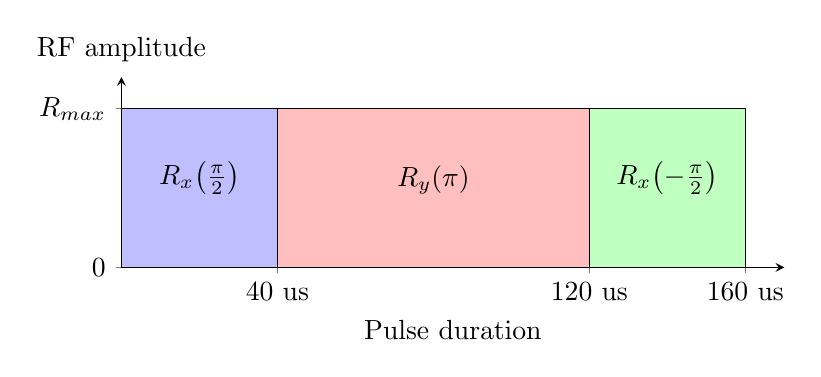
\begin{tikzpicture}[font=\normalsize]
\begin{axis}[
    width=10cm,
    height=4cm,
    xmin=0,xmax=17,
    ymin=0,ymax=3,
    axis lines=left,
    xlabel={Pulse duration},
    ylabel={RF amplitude},
    xtick={4,12,16},
    ytick={0,2.5},
    yticklabels={0,$R_{max}$},
    ylabel style={
    rotate=-90,
    at={(axis description cs:0,1.03)},
    anchor=south
},
    xticklabels={40 us, 120 us, 160 us},
    clip=false,
]

%--------------------------------------------------
% Rx(pi/2)
%--------------------------------------------------
\filldraw[fill=blue!25,draw=black]
(axis cs:0,0) rectangle (axis cs:4,2.5);

\node[above] at (axis cs:2,1){$R_x\!\left(\frac{\pi}{2}\right)$};

%--------------------------------------------------
% Ry(pi)
%--------------------------------------------------
\filldraw[fill=red!25,draw=black]
(axis cs:4,0) rectangle (axis cs:12,2.5);

\node[above] at (axis cs:8,1)
{$R_y(\pi)$};

%--------------------------------------------------
% Rx(-pi/2)
%--------------------------------------------------
\filldraw[fill=green!25,draw=black]
(axis cs:12,0) rectangle (axis cs:16,2.5);

\node[above] at (axis cs:14,1)
{$R_x\!\left(-\frac{\pi}{2}\right)$};



\end{axis}
\end{tikzpicture}
\caption{The example Euler angle rotation shown previously in Figure~\ref{fig:RxRyRx} can be implemented using only maximum amplitude hard pulses. The $R_x(\pi/2)$ rotation is a 40~\textmu s pulse with phase $0^\circ$, the $R_y(\pi)$ rotation is an 80~\textmu s pulse with phase $90^\circ$, and the final $R_x(-\pi/2)$ rotation is a 40~\textmu s pulse with phase $180^\circ$.}
    \label{fig:hardpulse_example}
\end{figure}

In this way, any arbitrary rotation of a single-spin state can be achieved using a finite number of hard pulses, by adjusting their phase and duration. This establishes hard pulses as a powerful tool for implementing single-spin rotations due to their short duration and high fidelity in the appropriate regime. As a result, they are often used to implement single-qubit rotation gates about the \(\hat{x}\), \(\hat{y}\), and \(\hat{z}\) axes, as well as the Hadamard gate, which can be represented as an effective \(\pi\)-rotation about the axis \(\frac{1}{\sqrt{2}}(\hat{x}+\hat{z})\).

\subsection{Multi-qubit operations}
\label{subsec:multi_qubit_operations}

For multi-qubit operations, the \(J\)-coupling term cannot be neglected as this inter-qubit interaction is used to mediate the transfer of information between the qubits involved. Since it is an always-on interaction, its effect on the system’s evolution must be taken into account over the entire duration of the control pulse. For a two-qubit system, the free evolution under just the \(J\)-coupling interaction, in the absence of a control pulse, is given by

\begin{equation}
    U(t)=e^{-iHt}=e^{-i2\pi J_{12}I_z^1I_z^2t}.
    \label{eq:J_coupling_evo}
\end{equation}

This represents a rotation by an angle of \(\theta =2\pi J_{12}t\), around the axis given by the operator \(I_z^1I_z^2\). This does not translate to a rotation around a single spatial axis like \(\hat{x}\), \(\hat{y}\), or \(\hat{z}\), but rather to a conditional phase evolution that depends on the state of the spins. Expanding the operator in terms of the Pauli operators for each spin yields

\begin{equation}
\begin{aligned}
    I_z^1\otimes I_z^2 &=\frac{1}{2}\begin{bmatrix}
        1 & 0 \\
        0 & -1 
    \end{bmatrix}\otimes I_z^2 \\&=\frac{1}{2}\left(|0\rangle\langle 0| \otimes I_z^2+|1\rangle\langle 1| \otimes -I_z^2\right).
    \label{eq:Jcoup_ZZoperator}
\end{aligned}
\end{equation}

The result is that the rotation axis is \(\hat{z}\) if the first qubit is in the state \(|0\rangle\), and \(-\hat{z}\) if it is in the state \(|1\rangle\). The same analysis can be performed for the second qubit.

This can be used for the analytical construction of multi-qubit gates such as the Controlled-NOT gate. This gate applies a NOT operation (an \(X\) gate) on the target qubit only when the control qubit is in the state \(|1\rangle\). Geometrically, this corresponds to a conditional \(\pi\)-rotation of the target qubit about the \(\hat{x}\)-axis on its Bloch sphere, conditioned on the state of the control qubit.

\begin{figure}[ht]
\centering
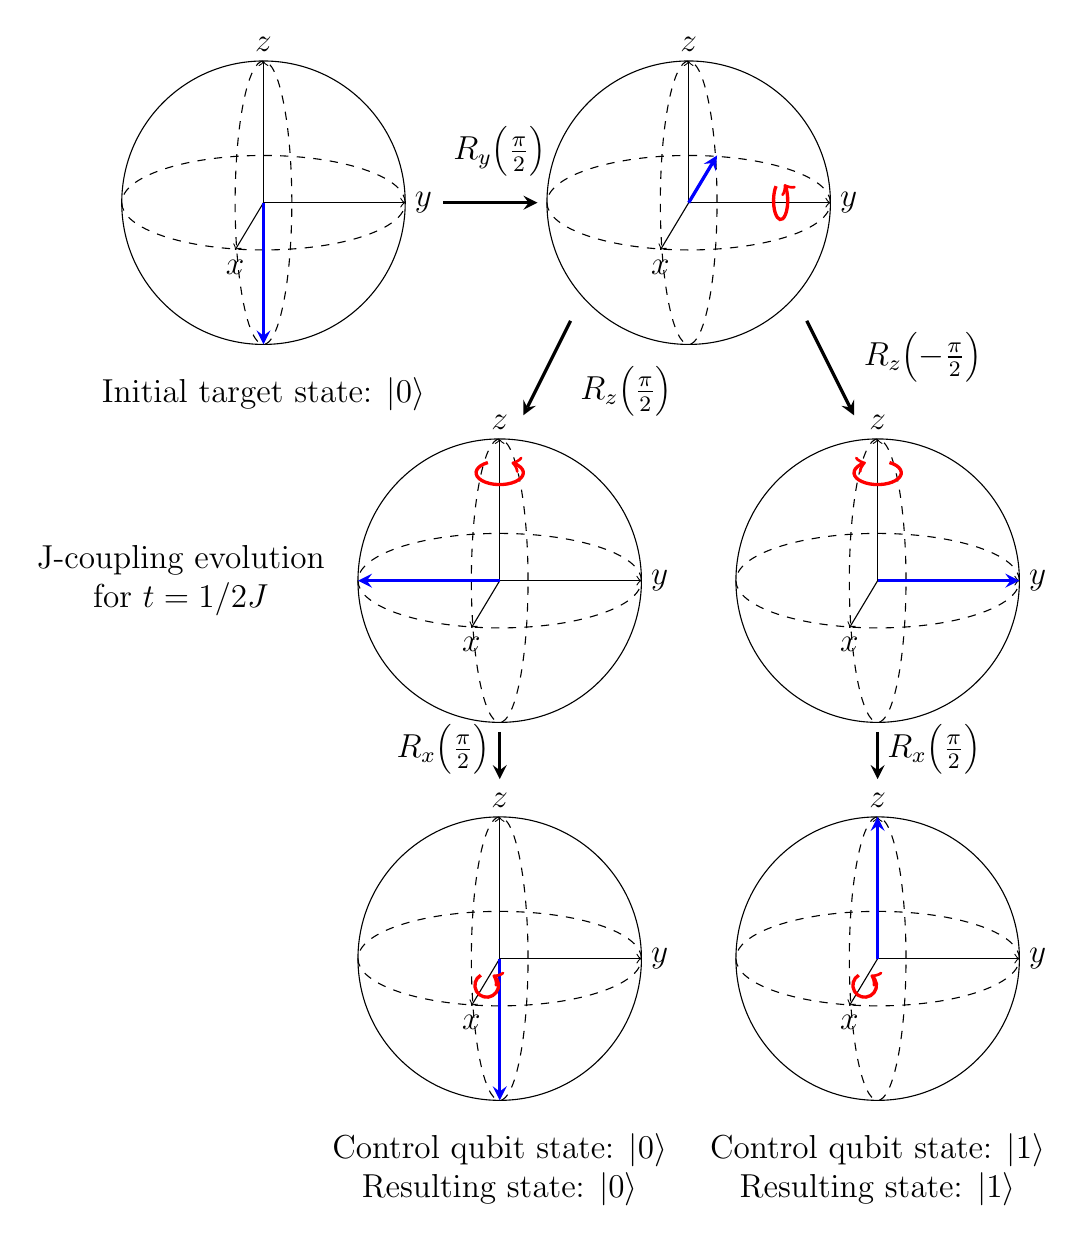
\begin{tikzpicture}[scale=0.6,font=\large]

\def\r{3}

%====================================================
% Sphere 0 : Initial state
%====================================================
\begin{scope}[shift={(-5,0)}]

% Sphere
\draw (0,0) circle(\r);
\draw[dashed] (0,0) ellipse ({\r} and {\r/3});
\draw[dashed] (0,0) ellipse ({\r/5} and {\r});

% Axes
\draw[->] (0,0)--(0,\r) node[above]{$z$};
\draw[->] (0,0)--(\r,0) node[right]{$y$};
\draw[->] (0,0)--(-\r/5,-\r/3) node[below]{$x$};

% State vector
\draw[very thick,blue,-stealth] (0,0)--(0,-\r);

\node[below] at (0,-\r-0.5)
{Initial target state: $|0\rangle$};

\end{scope}
%====================================================
% Sphere 1 : Ry(90)
%====================================================
\begin{scope}[shift={(4,0)}]

% Sphere
\draw (0,0) circle(\r);
\draw[dashed] (0,0) ellipse ({\r} and {\r/3});
\draw[dashed] (0,0) ellipse ({\r/5} and {\r});

% Axes
\draw[->] (0,0)--(0,\r) node[above]{$z$};
\draw[->] (0,0)--(\r,0) node[right]{$y$};
\draw[->] (0,0)--(-\r/5,-\r/3) node[below]{$x$};

% State vector
\draw[very thick,blue,-stealth] (0,0)--(\r/5,\r/3);

% Rotation arrow about y
\draw[red,very thick,->]
(1.85,0.35)
arc[start angle=130,end angle=420,
x radius=.15,
y radius=.4];

\end{scope}

%====================================================
% Sphere 2 : Rz(+pi)
%====================================================
\begin{scope}[shift={(0,-8)}]

\draw (0,0) circle(\r);
\draw[dashed] (0,0) ellipse ({\r} and {\r/3});
\draw[dashed] (0,0) ellipse ({\r/5} and {\r});

\draw[->] (0,0)--(0,\r) node[above]{$z$};
\draw[->] (0,0)--(\r,0) node[right]{$y$};
\draw[->] (0,0)--(-\r/5,-\r/3) node[below]{$x$};

% Rotated state
\draw[very thick,blue,-stealth] (0,0)--(-\r,0);

% Rotation arrow about z

\draw[red,very thick,->]
(-0.25,\r-0.5)
arc[start angle=120,end angle=420,
x radius=.5,
y radius=.25];

\node[left, align=center] at (-\r-0.5,0)
{J-coupling evolution\\
 for $t=1/2J$};

\end{scope}

%====================================================
% Sphere 3 : Rz(-pi)
%====================================================
\begin{scope}[shift={(8,-8)}]

\draw (0,0) circle(\r);
\draw[dashed] (0,0) ellipse ({\r} and {\r/3});
\draw[dashed] (0,0) ellipse ({\r/5} and {\r});

\draw[->] (0,0)--(0,\r) node[above]{$z$};
\draw[->] (0,0)--(\r,0) node[right]{$y$};
\draw[->] (0,0)--(-\r/5,-\r/3) node[below]{$x$};

% Final state
\draw[very thick,blue,-stealth] (0,0)--(+\r,0);

% Rotation arrow about z
\draw[red,very thick,->]
(0.25,\r-0.5)
arc[start angle=420,end angle=120,
x radius=.5,
y radius=.25];

\end{scope}

%====================================================
% Sphere 4 : Rx(pi/2)
%====================================================
\begin{scope}[shift={(0,-16)}]

\draw (0,0) circle(\r);
\draw[dashed] (0,0) ellipse ({\r} and {\r/3});
\draw[dashed] (0,0) ellipse ({\r/5} and {\r});

\draw[->] (0,0)--(0,\r) node[above]{$z$};
\draw[->] (0,0)--(\r,0) node[right]{$y$};
\draw[->] (0,0)--(-\r/5,-\r/3) node[below]{$x$};

% Final state
\draw[very thick,blue,-stealth] (0,0)--(0,-\r);

% Rotation arrow about x
\draw[red,very thick,->]
(-0.4,-0.35)
arc[start angle=120,end angle=420,
x radius=.25,
y radius=.25];

\node[below, align=center] at (0,-\r-0.5)
{Control qubit state: $|0\rangle$\\
    Resulting state: $|0\rangle$};

\end{scope}

%====================================================
% Sphere 5 : Rx(pi/2)
%====================================================
\begin{scope}[shift={(8,-16)}]

\draw (0,0) circle(\r);
\draw[dashed] (0,0) ellipse ({\r} and {\r/3});
\draw[dashed] (0,0) ellipse ({\r/5} and {\r});

\draw[->] (0,0)--(0,\r) node[above]{$z$};
\draw[->] (0,0)--(\r,0) node[right]{$y$};
\draw[->] (0,0)--(-\r/5,-\r/3) node[below]{$x$};

% Final state
\draw[very thick,blue,-stealth] (0,0)--(0,\r);

% Rotation arrow about x
\draw[red,very thick,->]
(-0.4,-0.35)
arc[start angle=120,end angle=420,
x radius=.25,
y radius=.25];

\node[below, align=center] at (0,-\r-0.5)
{Control qubit state: $|1\rangle$\\
    Resulting state: $|1\rangle$};

\end{scope}



%Arrows
% Sphere 0 -> Sphere 1
\draw[very thick,-stealth] (-1.2,0)--(0.8,0);
\node[above] at (0,0.35)
{$R_y\!\left(\frac{\pi}{2}\right)$};

% Sphere 1 -> Sphere 2
\draw[very thick,-stealth] (1.5,-2.5)--(0.5,-4.5);
\node[right] at (1.5,-4)
{$R_z\!\left(\frac{\pi}{2}\right)$};

% Sphere 1 -> Sphere 3
\draw[very thick,-stealth] (6.5,-2.5)--(7.5,-4.5);
\node[above right] at (7.5,-4)
{$R_z\!\left(-\frac{\pi}{2}\right)$};

% Sphere 2 -> Sphere 4
\draw[very thick,-stealth] (0,-11.2)--(0,-12.2);
\node[above left] at (0,-12.3)
{$R_x\!\left(\frac{\pi}{2}\right)$};

% Sphere 3 -> Sphere 5
\draw[very thick,-stealth] (8,-11.2)--(8,-12.2);
\node[above right] at (8,-12.3)
{$R_x\!\left(\frac{\pi}{2}\right)$};


\end{tikzpicture}
\caption{A CNOT gate can be implemented through a sequence of hard pulses making use of the intrinsic J-coupling evolution.  The target qubit is rotated to the transverse plane, where it evolves under the J-coupling interaction for a time \(t=1/2J\), which corresponds to a conditional \(\pi/2\) rotation about the \(\hat{z}\) or \(-\hat{z}\) axis.}
\label{fig:CNOT_bloch}
\end{figure}

However, deriving pulse sequences analytically for more complex operations or for systems with more than two qubits quickly becomes unmanageable. This is mainly due to the always-on nature of the \(J\)-coupling interaction, which cannot be switched off or modulated in strength. In addition, practical pulse design must account for the fact that a single hard pulse can unintentionally excite multiple spins simultaneously, making selective addressing and decoupling during gate implementation non-trivial.

\section{Numerical optimization}
\label{sec:numerical_optimization}

To circumvent the problems of analytical pulse design, especially in the presence of the aforementioned issues, numerical optimization methods are employed to systematically search for pulse parameters that achieve the desired quantum evolution with high fidelity.

Section~\ref{subsec:unitary_operation} established that an ideal quantum gate is described by a unitary operation. Consequently, the goal of a pulse optimization algorithm is to find the pulse parameters that maximize the similarity between the evolution generated by the pulse and the target unitary operation.

\subsection{Defining a cost function}
\label{subsec:cost_function}

Every numerical optimization algorithm begins with the definition of a cost function. The objective is to determine a set of parameters that either maximize or minimize this function.

In the present work, the cost function is defined as the \textbf{fidelity} of the quantum gate. It is computed by measuring the overlap between the target unitary operation and the unitary operation generated by the optimized pulse, making use of the Hilbert-Schmidt inner product, and normalized afterward:

\begin{equation}
    F = \frac{\left| \mathrm{Tr}(U_{target}^\dagger U_{optimized}) \right|^2}{d^2}.
    \label{eq:normalized_fidelity}
\end{equation}

It is important to distinguish between theoretical fidelity and experimentally achieved fidelity. The fidelity defined above is based on the assumption that the system dynamics behave exactly as described by the idealized Hamiltonian used during optimization (equation~\ref{eq:full_Hamiltonian}). However, this Hamiltonian is a product of multiple approximations and further experimental phenomena can lead to discrepancies between the optimized and implemented unitary operations.

The cost function can incorporate further objectives beyond fidelity, such as robustness and smoothness constraints. \textbf{Robustness} refers to the insensitivity of the optimized control pulse to small perturbations in system parameters, such as fluctuations in the magnetic field strength. This is incorporated into the cost function by evaluating the fidelity of the optimized pulse for a range of slightly perturbed Hamiltonians, and taking an average of the results.

\textbf{Smoothness} characterizes the temporal variation of the control amplitudes. Smooth control pulse profiles are encouraged because abrupt changes may not be faithfully reproduced by the experimental hardware due to finite bandwidth and transient rise-time effects, leading to discrepancies between the designed and implemented pulses.

In a similar vein, the optimized pulse can also be constrained to follow a \textbf{gaussian-square envelope}, which is a common pulse shape in NMR experiments. A smooth and physically realizable rise and fall time can be beneficial when considering the equipment's physical limitations, as well as that the optimized pulse will ideally be incorporated into a larger pulse sequence to form an algorithm.

In this work, the pulse envelope was implemented by performing a convolution of the pulse parameters with the desired envelope function, during the optimization process. However, it was later found through experimentation that this constraint was not necessary, as the experimental equipment was able to apply the optimized pulses faithfully.

\subsection{Optimization parameters}
\label{subsec:optimization_parameters}

Having characterized the cost function, the next step is the definition of the optimization parameters that will give shape to the optimized pulse. In Section~\ref{subsec:control_hamiltonian}, the control Hamiltonian was defined in terms of three parameters: the Rabi oscillation frequency \(\omega_1\), the RF field phase \(\phi_{rf}\), and the reference frame frequency \(\omega_{rf}\), in equation~\ref{eq:full_Hamiltonian}. In addition, the pulse duration \(t\) is also a parameter that can be controlled.

Under the lens of numerical optimization, these parameters are interpreted as the degrees of freedom that can be adjusted to maximize the cost function. The optimization parameters are therefore:

\begin{enumerate}
    \item \textbf{Detuning}: \(\delta_{rf}\)
    
    By varying the reference frame frequency \(\omega_{rf}\), the system can be driven off-resonance from the Larmor frequency \(\omega_0\) of the qubit, introducing a detuning term \(\delta_{rf} = \omega_{rf} - \omega_0\). In the rotating frame, this results in an additional effective \(z\)-component in the Hamiltonian, which modifies the rotation axis of the control field and, consequently, the efficiency and direction of the implemented operation.
    
    In homonuclear systems, this variation can be useful for achieving approximate single-qubit addressing and selective excitation. However, in heteronuclear systems such as the one used in this work, each qubit has a discernible Larmor frequency, making individual addressing straightforward.
    
    \item \textbf{Phase}: \(\phi_{rf}\)

    As a result of the description of the system by equation~\ref{eq:full_Hamiltonian}, the phase of the RF pulse dictates the axis of rotation of the unitary operation. A phase of \(\phi_{rf}=0\) defines a rotation about the \(\hat{x}\) axis, whereas a phase of \(\phi_{rf}=\pi/2\) defines a rotation about the \(\hat{y}\) axis.
    
    \item \textbf{RF field amplitude percentage}: \(R\)
    
    The amplitude of the RF field is defined relative to the maximum calibrated Rabi frequency of each qubit, corresponding to the maximum achievable RF amplitude. It is expressed as:
    
    \begin{equation}
        R = \frac{\omega_1}{\omega_1^{\mathrm{\max}}}
        = \frac{B_1}{B_1^{\mathrm{\max}}} \times 100\%
    \end{equation}
    
    The amplitude is directly related to the effective speed of the implemented unitary operation. Higher amplitudes are generally preferred, as they reduce the pulse duration required to perform the desired operation, thereby mitigating decoherence effects during long control sequences.
    
    \item \textbf{Pulse duration}: \(t\)
    
    The pulse duration represents the time required to implement the target unitary operation. As shorter duration pulses are always preferred to avoid decoherence in longer pulse sequences, the optimization process should aim to minimize this parameter whenever possible. Nevertheless, the minimum achievable pulse length is limited by the physical dynamics of the system, particularly the time required for inter-qubit interactions through \(J\)-coupling evolution.
    
\end{enumerate}

The total pulse duration is discretized into \(N\) time steps, within which the control parameters are held constant. Each optimized pulse therefore consists of an ordered sequence of hard pulses \(U_k\), whose parameters are adjusted such that the successive application of the corresponding elementary unitary operations approximates the target quantum gate.

\begin{equation}
\begin{gathered}
    U_k = e^{-iH(R^k,\omega_{rf}^k,\phi_{rf}^k)t^k} \\
    U_{\mathrm{optimized}} = U_N U_{N-1}\cdots U_2 U_1
\end{gathered}
\end{equation}

\begin{figure}[ht]
    \centering
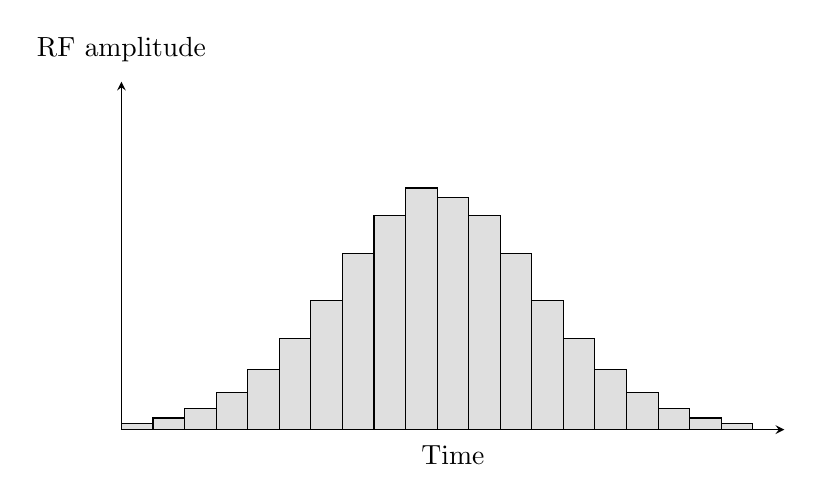
\begin{tikzpicture}[font=\normalsize]
\begin{axis}[
    width=10cm,
    height=6cm,
    xmin=0,xmax=21,
    ymin=0,ymax=9,
    axis lines=left,
    xlabel={Time},
    ylabel={RF amplitude},
    xtick={\empty},
    ytick={\empty},
    ylabel style={
    rotate=-90,
    at={(axis description cs:0,1.03)},
    anchor=south
},
    xticklabels={0,1,2,3,4,5,6,7,8,9,10},
    clip=false,
]

%--------------------------------------------------
% Pulses
%--------------------------------------------------
\addplot[
    ybar interval,
    fill=gray!25,
    draw=black
] coordinates {
    (0,0.15)
    (1,0.30)
    (2,0.55)
    (3,0.95)
    (4,1.55)
    (5,2.35)
    (6,3.35)
    (7,4.55)
    (8,5.55)
    (9,6.25)
    (10,6.00)
    (11,5.55)
    (12,4.55)
    (13,3.35)
    (14,2.35)
    (15,1.55)
    (16,0.95)
    (17,0.55)
    (18,0.30)
    (19,0.15)
    (20,0)
};

\end{axis}
\end{tikzpicture}
\caption{Pulse discretization. The continuous pulse is divided into \(N\) time steps. Within each time step, the control parameters are held constant, effectively resulting in a sequence of hard pulses, which are optimized to approximate the target unitary operation.}
    \label{fig:discretization}
\end{figure}


\subsection{Gradient Ascent Pulse Engineering}
\label{GRAPE}

To identify an optimal solution of a cost function, a common strategy is the use of gradient ascent and gradient descent algorithms. These methods compute the gradient of the cost function in parameter space and update the parameters in the direction of steepest increase or decrease of the cost function every iteration. The optimization is conducted iteratively until predefined convergence criteria are met, typically based on the magnitude of the gradient or the variation of the cost function between iterations.

An ordinary gradient based algorithm will obey the following workflow in Figure~\ref{fig:grape_flowchart}.

\begin{figure}[ht]
    \centering
    \begin{tikzpicture}[
    node distance=1.4cm,
    >=Stealth,
    every node/.style={font=\small},
    process/.style={
        rectangle,
        rounded corners,
        draw,
        minimum width=3.0cm,
        minimum height=0.9cm,
        align=center,
        fill=blue!15,
        draw=black
    },
    decision/.style={
        diamond,
        draw,
        aspect=2,
        align=center,
        inner sep=1pt,
        fill=red!15,
        draw=black
    },
    line/.style={->, thick}
]

% Nodes
\node[process] (guess) {Guess initial\\parameters};

\node[process, right=of guess] (unitary)
{Calculate resulting unitary\\and fidelity};

\node[decision, right=of unitary] (conv)
{Convergence\\ criteria met?};

\node[process, below=1.8cm of conv] (grad)
{Calculate gradient\\of the cost function};

\node[process, below=2.2cm of unitary] (update)
{Update parameters};

\node[right=0.8cm of conv] (end) {End};

% Main flow
\draw[line] (guess) -- (unitary);
\draw[line] (unitary) -- (conv);

\draw[line] (conv) -- node[above]{Yes} (end);

\draw[line] (conv) -- node[right]{No} (grad);
\draw[line] (grad) -- (update);

% Feedback loop
\draw[line]
(update) -- node[left]{New iteration} (unitary);

\end{tikzpicture}
    \caption{The algorithm begins with an initial guess of the control parameters, either arbitrary or based on prior knowledge of the system. The resulting unitary operation and its respective fidelity are computed as shown in equation~\ref{eq:normalized_fidelity}. If the convergence criteria are not met, the gradient of the cost function with respect to each of the control parameters is calculated after which the parameters are updated in the direction of the gradient. This process is repeated iteratively until the convergence criteria are satisfied.}
    \label{fig:grape_flowchart}
\end{figure}

As the system size increases, so does the complexity of its dynamics, as well as the number of parameters required to accurately describe them. Consequently, the associated computational cost of numerical optimization quickly becomes significant. In this context, one of the most widely used techniques for pulse design in \acl{nmr} is \acl{grape}. Introduced by Khaneja et al., \acs{grape} provides an efficient framework for solving a range of optimal control problems by enabling the systematic and computationally manageable optimization of control pulses~\cite{khaneja2005optimal}. Among the challenges it addresses is the design of control sequences that implement a desired unitary propagator, which is also the central objective of this work. The following description of the \acs{grape} algorithm is based on Khaneja et al.\cite{khaneja2005optimal}, in particular Section 2.4 of their work.

To efficiently explore the parameter space, a \acs{grape} algorithm begins by reparameterizing the control field from its polar representation, defined by an amplitude and phase, to a cartesian representation with independent control amplitudes along the orthogonal directions \(\hat{x}\) and \(\hat{y}\), denoted by \(R_x\) and \(R_y\). This parametrization ensures that the optimization variables have similar numerical behavior and avoids complications associated with the periodic nature of the phase parameter.

\begin{equation}
    R_x = R\cos\phi_{rf}
    \qquad
    R_y = R\sin\phi_{rf}
\end{equation}

\begin{equation}
    H_{k}=\sum_{i=1}^{n}2\pi\hbar\left(R_x^i \omega_1^{\mathrm{\max}} I_x+R_y^i \omega_1^{\mathrm{\max}} I_y\right)
    \label{eq:Hamiltonian_cartesian}
\end{equation}

Furthermore, for a radio frequency pulse divided into \(N\) time steps of duration \(\Delta t\), the control Hamiltonian at each time step \(j\), where \(H_0\) is the internal Hamiltonian of the system, \(H_k\) are the control Hamiltonians (in this case just the one in equation~\ref{eq:Hamiltonian_cartesian}), and \(u_k(j)\) are the control amplitudes to be optimized, is given by

\begin{equation}
    H_{\mathrm{control}}(j)=H_0+\sum_k u_k(j)H_k.
\end{equation}

Now, what distinguishes \acs{grape} from other optimization frameworks is the following step: at the beginning of each optimization iteration, the cumulative unitary evolution up to each time step and the corresponding backward-propagated target evolution are computed. The forward propagation is usually denoted by \(X_j\) and the backward propagation by \(P_j\).

\begin{equation}
\begin{aligned}
    P_j&=U_{j+1}^\dagger U_{j+2}^\dagger\cdots U_N^\dagger U_{target}\\
    X_j&=U_j U_{j-1}\cdots U_1
\end{aligned}
\end{equation}

These forward and backward propagators are then used to compute the gradient of the fidelity with respect to each control amplitude \(u_k(j)\), which quantifies how a small change in each of the parameters affects the final quantum gate's fidelity, and is given by

\begin{equation}
    \frac{\delta F}{\delta u_k(j)}=-2\mathrm{Re}\langle P_j|i\Delta t H_k X_j\rangle\langle X_j|P_j\rangle.
\end{equation}

Each control parameter \(u_k(j)\) is then updated in the direction of the gradient scaled by a factor \(\alpha\), known as step size or learning rate. This factor must be fine-tuned appropriately because a value that is too small leads to slow convergence and unnecessary computational expense, whereas a value that is too large may cause the optimization to overshoot and fail to converge to a local optimum. This will be discussed further in the following Section~\ref{optimizers}.

\begin{equation}
    u_k^{(m+1)}(j)=u_k^{(m)}(j)+\alpha\frac{\delta F}{\delta u_k(j)}
\end{equation}

After updating the control amplitudes, a new pulse sequence is obtained and the corresponding unitary operation and fidelity are recomputed. This process is repeated iteratively until a predefined convergence criterion is satisfied, typically a target fidelity or a maximum number of iterations. The result is a set of control amplitudes \(R_x(j)\) and \(R_y(j)\) defining a pulse sequence that maximizes the overlap between its unitary operator and the target quantum gate. 

The key insight that distinguishes \acs{grape} from other optimization frameworks is the reduced number of matrix exponential computations. By computing the forward and backward propagations only once per iteration, rather than once per parameter update, the computational cost is significantly reduced, enabling efficient optimization even for large-scale control problems.

\subsection{Function Optimizers}
\label{optimizers}

The optimization step of the algorithm, in which the parameters are updated based on the gradient scaled by a factor \(\alpha\), is particularly sensitive and must be carefully tuned. Rather than manually adjusting the learning rate, the use of more advanced optimization routines can lead to faster convergence and improved performance.

One such optimization algorithm is \textbf{\acl{lbfgs}~(\acs{bfgs})}, which is widely used in machine learning and optimal control for parameter estimation. It approximates second-order information by building an estimate of the inverse Hessian matrix, enabling efficient navigation of the parameter space toward a local minimum. The method is memory-efficient, as it stores only a limited number of vectors instead of the full Hessian matrix, making it well suited for problems with a large number of optimization parameters.

In this work, \acs{lbfgs} was the sole optimization algorithm used for generating control pulses using \acs{grape}.\@ However, one of its limitations is its susceptibility to convergence toward suboptimal local minima. When the cost function is represented by a complex landscape with multiple local minima, the optimizer may become trapped in non-optimal solutions, making it difficult to obtain high-fidelity results. To prevent this, a good initial guess that lies in the vicinity of an optimal solution is often required. Alternatively, more robust optimization algorithms can be used, which are less sensitive to local minima but typically require higher computational cost and slower convergence.

An alternative algorithm is \textbf{\ac{adam}}, a stochastic gradient descent method that combines momentum-based updates with adaptive learning rates. Each update is computed using an exponentially weighted average of past gradients and past squared gradients, which improves stability and reduces sensitivity to the choice of step size. The effective learning rate is automatically adapted at each iteration based on these moment estimates, leading to more robust convergence in complex optimization landscapes.